% Глава.	
\chapter{Лекция первая. Введение в БД.}

\section{Базы данных.}

\textit{БД} - это самодокументированная собрание интегрированных записей. Набор таблиц.

\textit{Самодокументированная} - хранятся метаданные, т.е. данные о данных.

\textit{Интегрированные записи} - Файлы данных. Целый комплекс. Имеются индексы. Метаданные

\section{Основные требования к БД.}
\begin{itemize}
	\item Не избыточность - не храним лишнюю информацию.
	\item Эффективность доступа - малое время отклика на действие пользователя.
	\item Совместное использование.
	\item Безопасность. Также внутренняя безопасность - защита от дурака (пример: вместо числа ввел букву).
	\item Восстановление после сбоя.
	\item Целостность - если ссылаемся на какой-то объект, то он должен быть. Не ссылаться на несуществеющие объекты.
	\item Независимость от сторонних приложений. Если программа отправляет ерунду БД должна обработать.
\end{itemize}

\section{СУБД, журнализация.}

\textit{СУБД} - (Средства управления БД) приложение, обеспечивающее создание, хранение, обновление
и поиск информации в БД.Программа.
\textbf{СУБД управляет БД}.

\textit{Система БД} - совокупность БД.

\textit{Транзакция} - набор действий, которые выполняются одновременно.
(Пример: онлайн перевод, одновременно в одном месте деньги ушли, в другом появились.)

\textit{Журнализация} - информация о действиях, которые происходили в системе. Помогает
в откате каких-то действий. \textbf{БД} сохраняет запросы в журнале.

\textbf{СУБД должна поддерживать языки.}

\section{Основные компоненты СУБД}

\begin{itemize}
	\item Ядро - управление памятью. Журнализация.
	\item Процессор языка БД - оптимизация. Выполнение.
	\item Подсистема поддержки времени исполнения.
	\item Сервисные программы - те утилиты, которые мы пишем, доп. возможность. (Вывод звездочек вокруг имени.)
\end{itemize}

\section{Классификация СУБД}

\begin{itemize}
	\item По модели данных
	      \begin{itemize}
		      \item Дореляционная.
		            \begin{itemize}
			            \item Инвертированный список (рис 1)
			            \item Иерархия. (Дерево)
			            \item Сетевые (граф)
		            \end{itemize}
		      \item Реляционная.
		      \item Постреляционная
	      \end{itemize}
	\item По архитектуре.
	      \begin{itemize}
		      \item Локальные - на одном устройстве.
		      \item Распространенные - на многих устройствах.
	      \end{itemize}
	\item По способу доступа к БД
	      \begin{itemize}
		      \item Файл-серверный подход - Подключились, взяли всё. Нагружаем клиента,
		            а не сервер. \textbf{Минусы: У каждого клиента своя копия.}
		      \item клиент-серверные - запросы выполняются на сервере, клиент получает
		            только нужное
		      \item Встраиваемые - маленькие базы, которые не нужны всем.
	      \end{itemize}
\end{itemize}

\chapter{Лабораторная работа 1.}

\section{Задание:}

\begin{itemize}
	\item Выбрать тему.
	\item Рисуем ER-модель нашей базы.
	\item Создать БД. Создать таблицу. (>= 3ёх объектов
	      (таблицы связки не считаются объектами)).
	      Создать ключи. (Все это в SQL-скрипт)
	\item Наполнить (csv) >= 1000 строк.
\end{itemize}

По итогу 2 фала: 1 SQL-скрипт и 1 модель.

\chapter{Семинар 1.}

\section{SQL}



\textit{SQL} - SQL (Structured Query Language – язык структурированных
запросов)\\
декларативный язык программирования, применяемый для создания, модификации и управления данными в реляционной базе данных.

SQL - работает в любой БД. В основах лежит реляционная модель.

В основе реляционной модели лежит теория множеств и логика предикатов.

T-SQL - нек-ое дополнение. Надстройка.

\begin{figure}[ht!]
	\centering{
		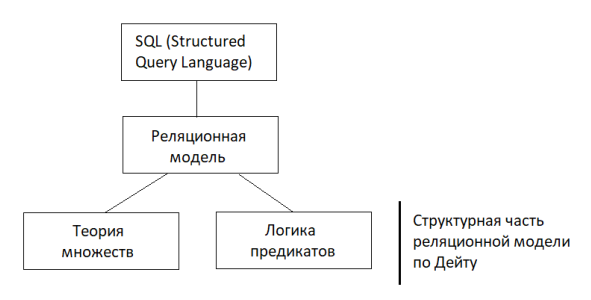
\includegraphics[width=0.6\textwidth]{01.png}
		\caption{SQL}}
\end{figure}

\textit{Заголовок} – набор атрибутов (В SQL - столбцы), каждый из которых имеет определенный
тип.\\
\textit{Атрибут} – совокупность имени и типа данных (Атрибут==столбец).Атрибут – название столбца, его тип + дополнительные настройки\\
\textit{Тело} – множество картежей (В SQL – строки).\\
\textit{Заголовок} кортежа – заголовок отношения.

\begin{figure}[ht!]
	\centering{
		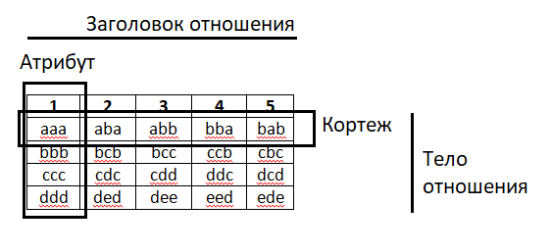
\includegraphics[width=0.6\textwidth]{02.png}
		\caption{Пример таблицы.}}
\end{figure}

\section{Основные языки}
Логику работы с данными можно разделить на три основных языка:
\begin{itemize}
	\item DLL (\textit{Data Definition Language}) - (Создаем объекты для хранения данных).Служит для описания структуры БД:
	      \begin{itemize}
		      \item Создать (Create)
		      \item Удалить (Drop)
		      \item Изменить (Alter)
	      \end{itemize}


	\item DML  (\textit{Data Manipulation Language}) -  Язык для работы с данными
	      \begin{itemize}
		      \item Обновить (update)
		      \item Загружать (insert)
		      \item Удалять (delete/truncate)
		      \item Читать (select)
	      \end{itemize}

	\item DCL (\textit{Data Control Language}) - Служит для управления доступа к объектам.
	      \begin{itemize}
		      \item Выдача прав доступа к объекту (grand)
		      \item Удаление прав доступа на объект (revoke)
	      \end{itemize}
\end{itemize}

Обращение к таблице.
Схема обращения к таблице:
[название БД].[название схемы].Название таблицы. Рис. \ref{fig:ref1}


\begin{figure}[ht!]
	\centering{
		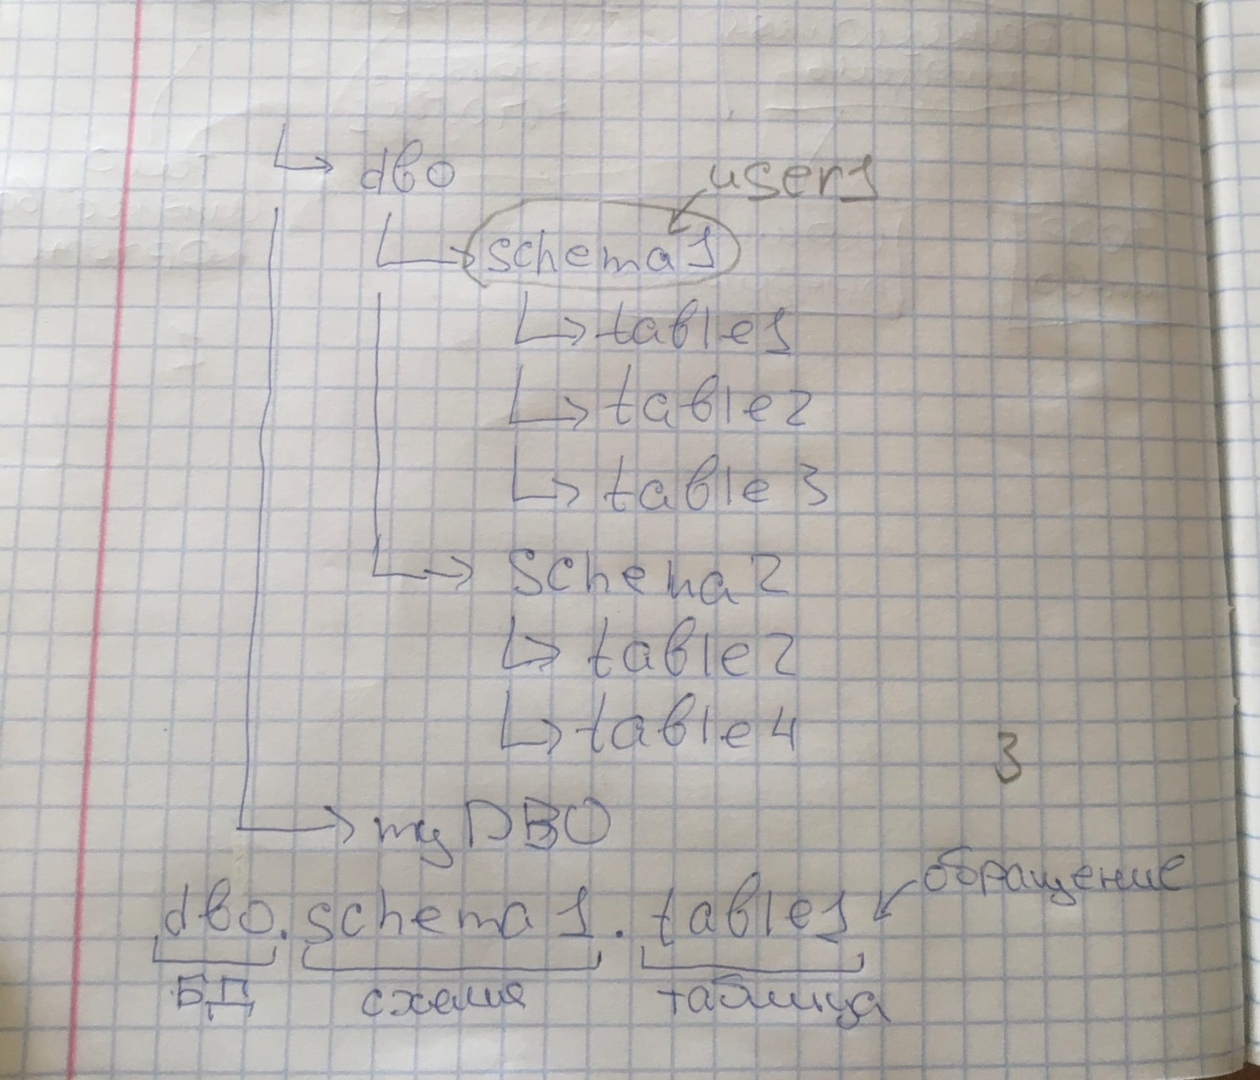
\includegraphics[width=0.6\textwidth]{03.jpg}
		\caption{Структура БД.}
		\label{fig:ref1}}
\end{figure}

\section{Способы хранения данных}

\begin{itemize}
	\item Таблица (table).
	\item Временные таблица (temp table). По завершению сессии таблица удаляется.
	\item Представление (View)
	\item Производные таблицы. (Временная)
	\item Индексированное представление.
\end{itemize}

\textbf{Пример создания таблицы}

\lstset{language=SQL}
\begin{lstlisting}
CREATE TABLE dbo.EmployeePhoto
(
Id int IDENTITY(1, 1),
EmployeeId int NOT NULL PRIMARY KEY,
Photo varbinary(max) FILESTREAM NULL,
MyRowGuidColumn uniqueidentifier NOT NULL ROWGUIDCOL
UNIQUE DEFAULT NEWID()
);
\end{lstlisting}

% \lstinputlisting{src/create.sql}

id - АТРИБУТ типа int счетчик шагаем начиная с единицы с шагом 1.\\
Employer id - поле, которое используем в кач-ве идентификатора.\\
Photo - По умолчанию NULL - пустой.\\
MyRawGuidColumn - Уникальное, DEFAULT - по умолчанию поле задается newID.\\
nvarchar -  Выделяет столько памяти, какова длина строки\\
varchar - Физически занята вся строка. Занято пробелами.\\
Salary - numeric(15, 2) - Сколько всего цифр выделено в нашем числа, сколько знаков
после запятой.\\

% create view v_workers as
% select id.Fio
% from workers

% \textbf{Удаление:}

% % \lstset{language=SQL}
% % \begin{lstlisting}

% % \end{lstlisting}

% \lstset{language=SQL}
% \begin{lstlisting}

% \end{lstlisting}

% drop table workers\\

% Ограничения
% Alter table "Деталь-Поставщики" add constraint My_Fr_constr 
% foreign key(id_n, name) в скобках атрибуты  "Деталь-Поставщики"
% references "Поставщики" (id_n, name);
% Добавляем новые эл-ты в сущ-ую конструкцию.
% Создает  ограничение, которое ссылает (id_n, name) на (id_n, name) Деталь-Поставщики

% Добавление. (Добавляем детали в коробках).
% alter table "Детали" add edumn Qty int;
% Удаление
% alter table "Детали" drop column Qty;

% Изменение. (Атрибута)
% alter table "Детали" modify column Qty to cnt;

% Переименование самого объекта. (Таблицы)
% alter table "Детали" rename to "Детали_dd"

% Переходим к DML.\\
% Select. Запрос\\
% from\\
% where\\
% group by\\
% having\\
% order by\\

% Вывод на экран.
% select * (выбрать всё)
% from "Детали"

% select id, name
% from "Детали"

% select id as "ID Детали", name
% from "Детали"


% where <Предикат> (Предикат true/false)
% * Предикат сравнения =,>,<,>=,<=,!=,<>
% select *
% from "Детали"
% where name="гвоздь"
% (Выбрать все, где поле name="гвоздь")

% * Предикат Between
% where id Between 3 and 5
% (Выведет все id в пределах от 3 до 5)

% * Предикат LIKE
% \% - >=0 символов
% \_ = 1 символ
% select *
% from "Детали"
% where name LIKE "Г\%"
% (Выведет имена с буквой г и >=0 символов)
% Чувствительный к регистру, поэтому мы можем сделатль так:
% upper(name), или так lower(name)

% * Предикат IN - ищем атрибуты, которые входят в какой-то список (массив)
% select *
% from "Детали"
% where color in ("К","С") <- в скобках также может быть запрос. Результатом будет множество кортежей.

% * Предикат is [not] null
% where color=null (Нельзя так, null != null. Вернет только шапку)
% Нужно так:
% where color is null